\documentclass[a4paper]{article}
%\usepackage{algorithmicx}
\usepackage{algorithm}
\usepackage{algpseudocode}
\usepackage{amsfonts}
\usepackage{amsmath,amssymb}
\usepackage{graphicx}
\usepackage{hyperref}
\usepackage[htt]{hyphenat}
%\usepackage{media9}
\usepackage{minted}
%\usepackage{movie15}
\usepackage{nicefrac}
\usepackage{siunitx}
\usepackage{tabto}

% Math symbols
\newcommand{\mt}{\ensuremath{\mathsf{T}}}  % transpose
%\newcommand{\m}[1]{\ensuremath{\mathrm{\mathbf{#1}}}}  % matrix, vector
\newcommand{\m}[1]{\ensuremath{\mathtt{#1}}}  % matrix, vector
\newcommand{\col}{\ensuremath{\mathrm{col}}}  % column vector
\newcommand{\s}[1]{\ensuremath{\mathrm{\mathcal{#1}}}}  % set
\newcommand{\subjectto}{\ensuremath{\mathrm{s.t.}\ }}
\newcommand{\reals}{\mathbb{R}}

\newcommand{\etal}{\emph{et al.}}

\newcommand{\code}[1]{\texttt{#1}}
\DeclareTextFontCommand{\bf}{\bfseries}

\DeclareMathOperator*{\argmin}{argmin}
\DeclareMathOperator*{\argmax}{argmax}

\newcommand{\python}[1]{\mintinline{python}{#1}}
\newcommand{\file}[1]{\mintinline{bash}{#1}}
%\newcommand{\file}[1]{\verb|#1|}
%\newcommand{\file}[1]{\PVerb[]{#1}}
%\newcommand{\file}[1]{\emph{\replunderscores{#1}}}

\makeatletter
% \expandafter for the case that the filename is given in a command
\newcommand{\replunderscores}[1]{\expandafter\@repl@underscores#1_\relax}

\def\@repl@underscores#1_#2\relax{%
    \ifx \relax #2\relax
    % #2 is empty => finish
    #1%
    \else
    % #2 is not empty => underscore was contained, needs to be replaced
    #1%
    \textunderscore
    % continue replacing
    % #2 ends with an extra underscore so I don't need to add another one
    \@repl@underscores#2\relax
    \fi
}
\makeatother

%\setmintedinline{breaklines}

\title{
Frontier-based Exploration---Semestral Work\\
%Robotic Exploration in Simulated Environment\\
\vspace{0.25em}
\Large Autonomous Robotics
}
\author{Tom{\'a}{\v s} Pet{\v r}{\'i}{\v c}ek}
\date{\today}

\begin{document}

\maketitle


\section{Assignment}

The semestral work will be carried out individually (no teams), using a simulator instead of the real robots in the labs.
%You can use tools for remote collaboration of your choice.
Remote access to the lab computers is provided to all students (see below).
The task is to design and implement a system which performs autonomous exploration of an unknown environment using a single robot.
%, covering as much of the environment as possible.

The system will be assigned score based on the amount of empty space it covers,
by comparing the \href{http://docs.ros.org/melodic/api/nav_msgs/html/msg/OccupancyGrid.html}{occupancy grid} messages published at the
%\mintinline{bash}{/occupancy}
\file{/occupancy}
topic to the ground-truth.
Namely, the true empty cells which are marked as empty in the published occupancy grid count as positive points and the true occupied and unobservable cells which are marked as empty count as negative points.
Letting $o_i$ be the occupancy values in the
%\mintinline{bash}{/occupancy/data}
\file{/occupancy/data}
array, $o_i \in \{-1, 0, 1, \ldots, 100\}$, values $0 \le o_i < 25$ will be considered empty%
\footnote{You can set similar thresholds for planning and frontier detection as you like.
This threshold will be used solely for the evaluation.}
($-1$ means unknown).

%SLAM, frontier identification, path planning, and high-level exploration control must be provided.
You should use components and nodes you have implemented previously, possibly modifying and improving them as necessary.
%Nevertheless, you can improve and modify them as necessary.
The main task will be to design and implement a brand-new ROS node for high-level planning and control of the whole exploration process.
The node---executable Python script---should be located at \file{exploration/scripts/explorer}.
An empty template is provided in the student package (see below).
%It can already be run%
%\footnote{\mintinline{bash}{rosrun exploration explorer [<arguments>]}}
%but won't do anything until you implement it.
%A possible high-level operation of such a node is described in Alg.~\ref{alg:exploration} below.
Alg.~\ref{alg:exploration} below provides an overview of a possible implementation.
An exploration experiment with such a node is shown in Fig.~\ref{fig:exploration}.
%\begin{algorithm}[tb]
%\caption{Exploration node---overview of a possible implementation}
%\begin{algorithmic}[1]
%\While{any frontier left} \Comment \emph{frontier.py}
%\State Pick a frontier. \Comment \emph{frontier.py}
%\State Plan a path to the frontier. \Comment \emph{planner.py}
%\State Delegate execution to low-level control. \Comment \emph{path\_follower}
%\State Monitor execution of the plan.
%\State Invoke a recovery behavior if needed. \Comment \emph{path\_follower}
%\EndWhile
%\end{algorithmic}
%\label{alg:exploration}
%\end{algorithm}

\begin{algorithm}[tb]
\caption{Exploration node---overview of a possible implementation}
\begin{algorithmic}[1]
\State Pick a frontier, if any, or a random position as a goal. \Comment \file{frontier.py}
\State Plan a path to the goal, or go to line 1 if there is no path. \Comment \file{planner.py}
\State Delegate path execution to low-level control. \Comment \file{path_follower}
\State Monitor execution of the plan.
\State Invoke a recovery behavior if needed. \Comment \file{path_follower}
\State Repeat from line 1.
\end{algorithmic}
\label{alg:exploration}
\end{algorithm}

\begin{figure}[tb]
\centering
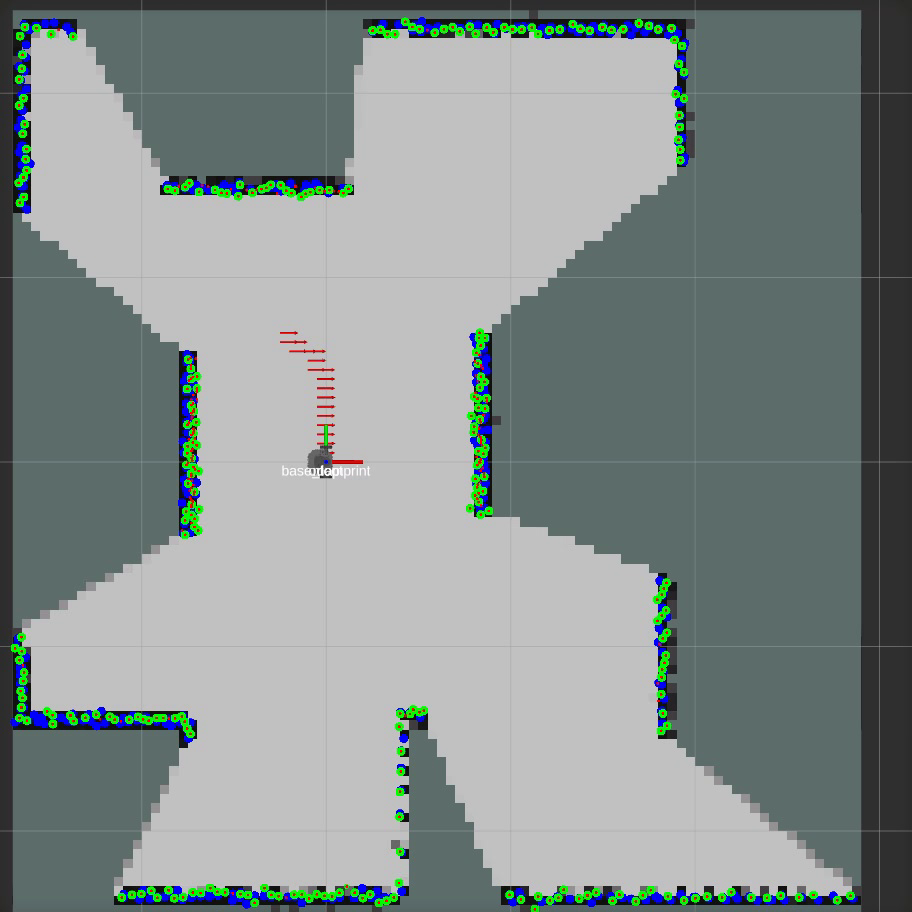
\includegraphics[width=0.24\textwidth]{exploration-stage_4-00080}%
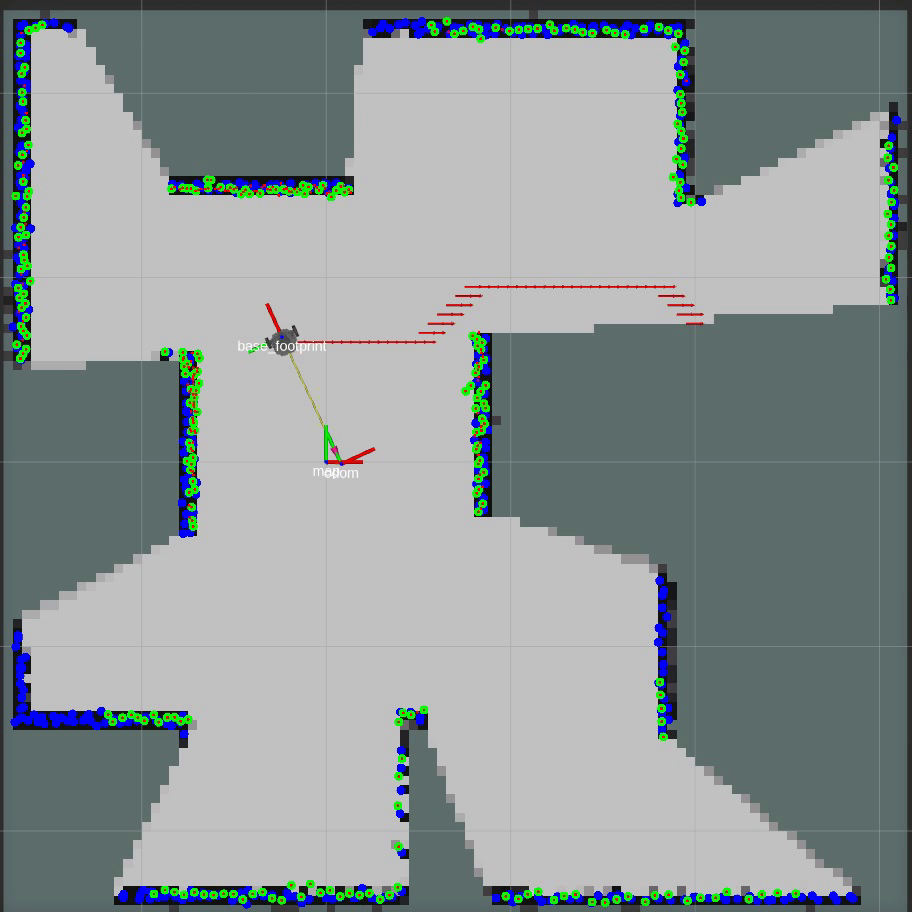
\includegraphics[width=0.24\textwidth]{exploration-stage_4-00218}%
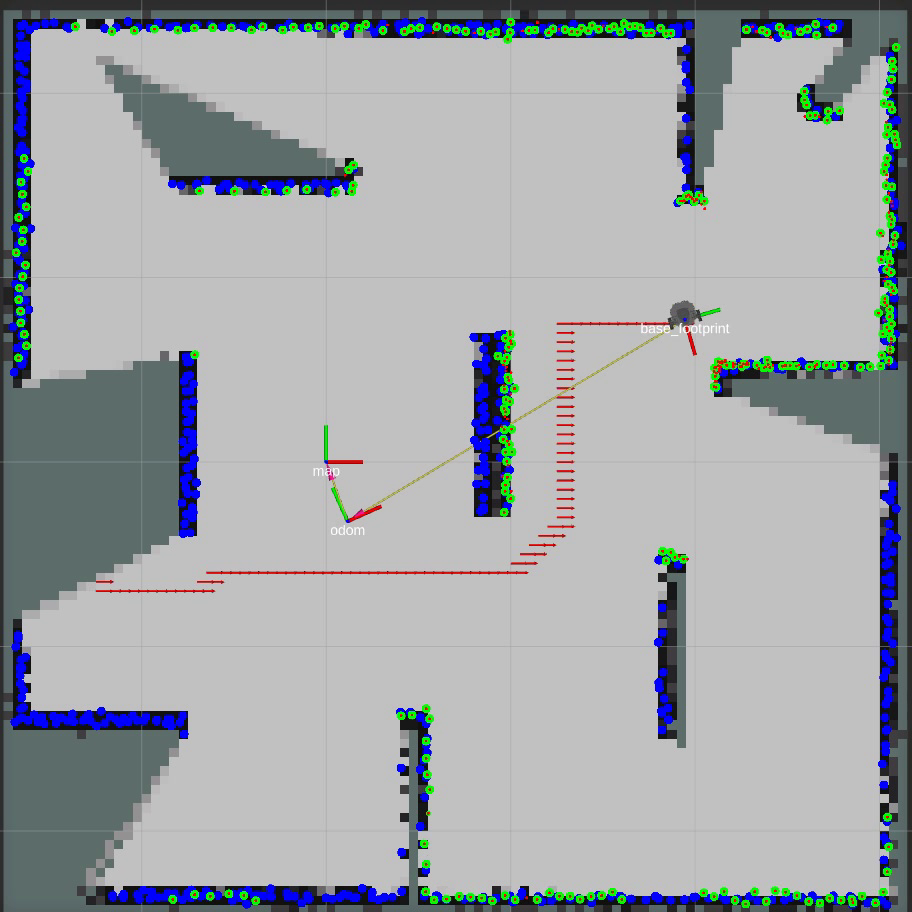
\includegraphics[width=0.24\textwidth]{exploration-stage_4-00485}%
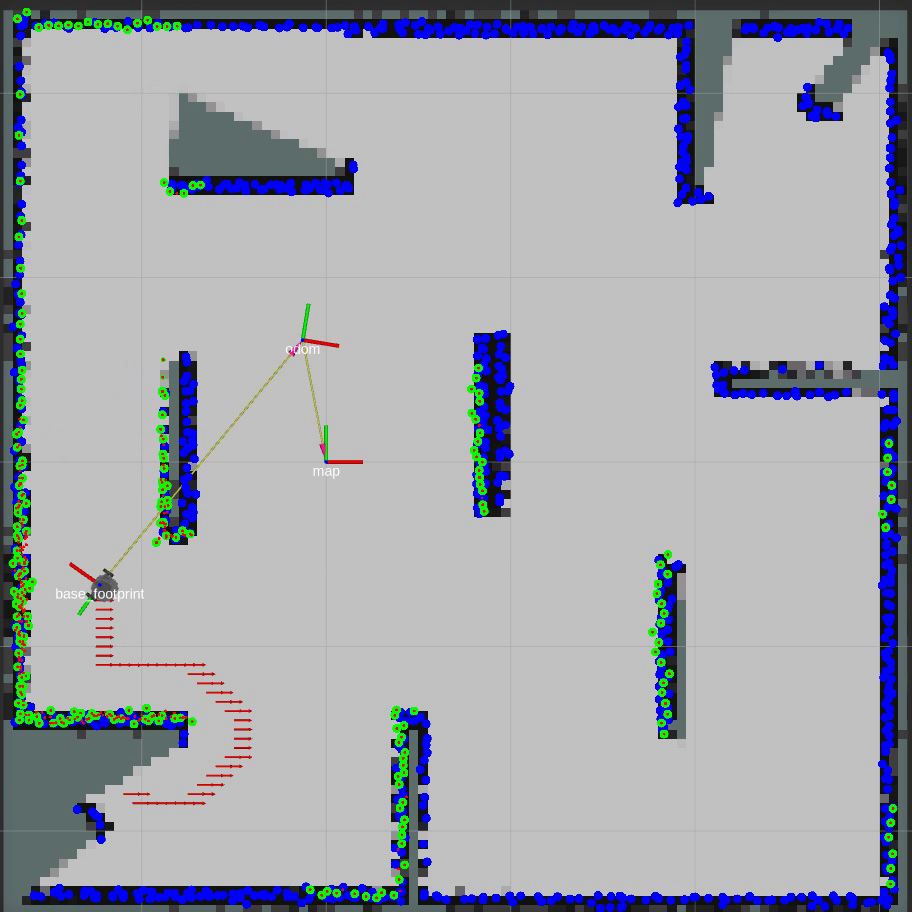
\includegraphics[width=0.24\textwidth]{exploration-stage_4-00830}%
\caption{An exploration experiment in \emph{stage\_4}.
It shows four successively planned and executed exploration paths.
Each path consists of multiple poses depicted as small red arrows.
Only path positions were planned and later followed, the visualized arrow orientations have no meaning.
Black grid cells correspond to occupied cells, light gray to empty cells.
The red, blue, and green points correspond to the measurements, the point map, and the registered points, respectively, from the \file{icp_slam_2d} node.
See the \href{https://cw.fel.cvut.cz/b192/_media/courses/aro/tutorials/exploration-stage_4.ogv}{video} with the full experiment.
}
\label{fig:exploration}
\end{figure}

\subsection{ROS Nodes}

The following ROS nodes participate in exploration.
\begin{itemize}\itemsep0em
\item \file{aro_slam/scripts/icp_slam_2d} uses (your) \file{aro_slam.icp} module and provides localization and mapping---including the occupancy grids which undergo evaluation.
\item \file{exploration/scripts/frontier.py} (yours) provides services related to finding frontiers. (UPDATED: Note the small changes, e.g. adding the \python{robot_frame} parameter.)
\item \file{exploration/scripts/planner.py} (yours) provides a path planning service. (UPDATED: Note the small changes, e.g. adding the \python{robot_frame} parameter.)
\item \file{exploration/scripts/explorer} (yours, to be implemented) provides high-level exploration planning and control.
\item \file{exploration/scripts/path_follower} (provided, new) provides a low-level (proportional) motion control, executing paths published by \file{explorer}.
The node always acts upon the last received path.
An empty path means stopping the robot.
Without remapping it listens for \file{exploration}\allowbreak\file{/}\allowbreak\file{Path} messages at topic \file{path}.

In the control loop, it first finds the closest point on the path and navigates towards the waypoint \python{look_ahead} steps ahead of this closest point.
In other words, it does not maintain any history of what has been covered.
As a result, having loops in the path may not work as expected---loops may be skipped or may be repeated indefinitely.
The motivation was to keep the node as robust and simple as possible and to ease custom modifications, if these turn out to be necessary to handle the planned paths.

With parameter \python{use_path_theta} set to \python{'none'}, as in the provided launch file, orientation from individual poses is neglected and the robot is oriented towards the waypoint, eventually keeping whatever orientation it had when reaching the goal.
That should be sufficient for successful exploration.
Setting the parameter to \python{'last'} makes it use orientation of the last pose only.%
\footnote{Currently, setting \python{'all'} is also possible (the node won't complain) but will not work without many additional changes.
Besides other things, there is an interplay with the \python{look_ahead} parameter.}
%On reaching the goal, it clears its path.
\end{itemize}

\subsection{Simulation Environment}

Configuration and launch files with the simulated environment are provided in separate package \file{aro_sim}.
There are few changes in the sensor configuration from the defaults provided by \file{turtlebot3} packages.
Namely, the source for the odometry are wheel encoders instead of ground-truth pose.
As a result, the odometry must be corrected in SLAM, otherwise the localization would be inaccurate.
We have also increased lidar range (to $\SI{10}{m}$) and noise level.

Tampering with the simulation environment during evaluation is prohibited and will be penalized.

\subsection{Evaluation}

Score will be accumulated from multiple experiments, varying worlds and starting positions.
The evaluation will be done on worlds similar to \file{stage_3}, \file{stage_4}, and \file{world}.
They won't contain open areas as in \file{house}.
A possible addition will be more maze-like with longer corridors and thick walls.
Only the \file{burger} robot will be used in evaluation.

Please note that we will evaluate performance of the whole system in terms of the published occupancy grids, so the nodes must not only work individually but also work well with other nodes to fulfill their role in the whole system.
Things to consider:
\begin{itemize}\itemsep0em
\item Inaccurate localization will result in distorted maps and wrong cells being compared to the ground truth.
\item Slow localization will have a negative impact on low-level motion control.
Low-level motion control can be adjusted as well if needed.
\item As all experiments are run in simulator, possible recovery behaviors can be quite aggressive.
Nevertheless, if the maneuvers are too aggressive and robot is hitting obstacles, it will adversely affect odometry and initial pose estimates for ICP.
\item Choosing inappropriate goals a visiting already covered areas repeatedly will slow down exploration.
\item Having no recovery or fallback behaviors can lead the system to halt in the very beginning.
\end{itemize}
A general advice is to focus on performance bottlenecks.

More details of the evaluation procedure will be announced later.

 
\section{Remote Access to Labs}

Students can use lab computers (E-130, E-132, E:230) remotely, including remote desktop.
We suggest using remote desktop via \href{https://xpra.org/}{Xpra}---see the \href{https://cw.fel.cvut.cz/b192/courses/aro/tutorials/remote_access}{brief how-to} at the course website.

If needed, more information can be found in
\begin{itemize}\itemsep0em
\item the \href{https://www.thewoodcraft.org/pub/hornilouka/videa/}{video tutorials} (in Czech and English) and
\item the \href{https://support.dce.felk.cvut.cz/mediawiki/index.php/Vzd%C3%A1len%C3%BD_p%C5%99%C3%ADstup_do_laborato%C5%99%C3%AD}{user guide} (only Czech).
\end{itemize}
 
\section{Workspace Configuration}

The simulation environment has been tested on Ubuntu 18.04 with ROS Melodic, using both a generic Ubuntu installation and the provided Singularity image below.
Other configurations will not be supported.

\subsection{Robolab Singularity Image}

This
\href{http://ptak.felk.cvut.cz/tradr/share/robolab_melodic.simg}{Singularity image} (UPDATED: April 22 2020)
is used at the labs---it already provides all the dependencies.
To enter the shell within the Singularity image:
\begin{minted}{bash}
singularity shell /path/to/robolab_melodic.simg
\end{minted}
In the labs, there is also an expanded image available for convenience:
\begin{minted}{bash}
singularity shell /opt/singularity/robolab/melodic
\end{minted}

To build your customized image, use the scripts from the \href{https://gitlab.fel.cvut.cz/robolab/deploy}{Robolab deploy repository}.

\subsection{Catkin Workspace}

The workspace can then be configured as follow:
{
\small%
\begin{minted}{bash}
ws=~/workspace/aro
mkdir -p "${ws}/src"
cd "${ws}/src"
curl -sSL https://cw.fel.cvut.cz/b192/_media/courses/aro/tutorials/aro_sim.zip -O
unzip *.zip
cd "${ws}"
catkin init
catkin config --extend /opt/ros/aro
catkin config --cmake-args -DCMAKE_BUILD_TYPE=Release
catkin build -c
\end{minted}
}

\subsection{Extras for a Generic Ubuntu}

On a generic Ubuntu with ROS Melodic (not with the Singularity image above), dependencies must be install prior \file{caktin build -c} from the accompanied rosinstall file and via \href{http://wiki.ros.org/rosdep}{rosdep}.
{
\small
\begin{minted}{bash}
cd "${ws}/src"
wstool init
wstool merge aro_slam/dependencies.rosinstall
wstool up -j 4
cd "${ws}"
rosdep install --rosdistro melodic --from-paths src --ignore-src -r -y
\end{minted}
}

Also note that we will use Gazebo 9.13 during evaluation instead of Gazebo 9 from the default Ubuntu repository.
Gazebo 9.13 is provided by the Open Source Robotics Foundation and may be installed using the
\href{https://gitlab.fel.cvut.cz/robolab/deploy/-/blob/master/scripts/install_gazebo}{installation script}
from the
\href{https://gitlab.fel.cvut.cz/robolab/deploy}{robolab deploy}
repository.

\section{Package Usage}
Don't forget to source your workspace:
\begin{minted}{bash}
source "${ws}/devel/setup.bash"
\end{minted}
To run the whole system inside the simulated environment:
\begin{minted}{bash}
roslaunch aro_sim turtlebot3.launch world:=stage_4
\end{minted}
Worlds worth trying are \file{stage_3}, \file{stage_4}, \file{world}, and \file{house}.

All your nodes should be configured for evaluation within launch file\\
\file{exploration/launch/exploration.launch}
which is included from launch file
\file{aro_sim/launch/turtlebot3.launch}
above.


%\bibliographystyle{IEEEtran}
%\bibliography{/home/petrito1/bib/petricek}

\end{document}
